\documentclass{article}
\usepackage[utf8]{inputenc}

\title{EE568 Project 3 - PM Motor Comparison Analysis}
\author{by Hakan Saraç - 2408086}
\date{}



\usepackage{natbib}
\usepackage{graphicx}
\usepackage{indentfirst}
\usepackage{siunitx}
\usepackage{svg}
\usepackage{hyperref}


\addtolength{\oddsidemargin}{-.875in}
\addtolength{\evensidemargin}{-.875in}
\addtolength{\textwidth}{1.75in}
\addtolength{\topmargin}{-.875in}
\addtolength{\textheight}{1.75in}    
\begin{document}

\maketitle

\newpage
\section{Introduction}
In this project, we will examined some stuff.

\section{Question 1 - Magnetic Loading}
\subsection{Part - a}

Flux path for one pole pair is provided in Figure \ref{fig:FluxPath} and the corresponding equivalent magnetic circuit is provided in Figure \ref{fig:MagneticCircuit}. In this part, the permeability of the rotor and stator are assumed to be infinite. Therefore, the reluctance of core material becomes zero. Another assumption can be made as that there is no fringing or leakage flux and flux lines are straight as shown in Figure \ref{fig:FluxPath} with green lines. \newline
The machine parameters are as follows:
\begin{itemize}
    \item Number Of Poles: 4
    \item Motor Axial Length: 100 mm
    \item Air Gap Clearance: 1 mm
    \item Magnet To Pole Pitch Ratio: 0.8
    \item Rotor Diameter: 100 mm
    \item Magnet Thickness: 4 mm
    \item Magnet Type: NdFeB N42 grade (ur=1.05), radial shaped
\end{itemize} 
\bigskip
\noindent With the assumptions made, the reluctance $R_{m1}$ and $R_{m2}$ in Figure \ref{fig:FluxPath} can be calculated as:

\begin{equation} \label{eqn:PoleAreaFormula}
    A_{pole} = \frac{\pi*D_i*L_{axial}}{P}=0.007853 \: \mathrm{m^2}
\end{equation}
where P is the number of poles.

\bigskip


\noindent From the magnet to pole pitch ratio value of 0.8 (shown as $K$ in (\ref{eqn:MagnetAreaPerPole})), the magnet area per pole can be calculated. 
\bigskip

\begin{equation} \label{eqn:MagnetAreaPerPole}
    A_{magnetperpole} = A_{pole}*K = 0.006283 \: \mathrm{m^2}
\end{equation}

\begin{equation} \label{eqn:NonMagnetAreaPerPole}
    A_{nonmagnetperpole} = (1-K)*A_{pole} = 0.00157 \: \mathrm{m^2}
\end{equation}

\begin{equation} \label{eqn:MagnetReluctance}
    R_{m1}  =  R_{m2} =  \frac{H_{magnet}}{A_{nonmagnetperpole}*\mu_0*\mu_r}  = 482480 \: \mathrm{\frac{1}{Henry}} 
\end{equation}

\begin{equation} \label{eqn:MagnetReluctance}
    R_{ag1}  =  R_{ag2} =  \frac{H_{airgap}}{A_{magnetperpole}*\mu_0}  =  126650  \: \mathrm{\frac{1}{Henry}} 
\end{equation}

\begin{equation} \label{eqn:MmfPerMagnet}
    \mathcal{F}_{permagnet} = A_{magnetperpole}*B_{residual}*R_{m1} = 4001.61 \: \mathrm{Amperes}
\end{equation}

\bigskip

\noindent Assuming that the core is infinitely permeable, loop equation of the equivalent circuit (see Fig.\ref{fig:MagneticCircuit}) results in (\ref{eqn:AirGapFlux}).
\bigskip

\begin{equation} \label{eqn:AirGapFlux}
    \phi_{m} = \frac{2*\mathcal{F}_{permagnet}}{R_{m1}+R_{m2}+R_{ag1}+R_{ag2}} = 0.00657 \: \mathrm{Weber}
\end{equation}

\begin{equation} \label{eqn:AirGapFluxDensity}
    B_{m} = \frac{\phi_{m}}{A_{magnetperpole}} = 1.0455 \: \mathrm{Tesla}
\end{equation}

\noindent From the values found in (\ref{eqn:AirGapFluxDensity}), the magnetic field strength value is provided in (\ref{eqn:MagneticFieldStrength}).
\begin{equation} \label{eqn:MagneticFieldStrength}
    H_m = \frac{B_m-B_{residual}}{\mu_r*\mu_0} = -208004.48 \: \mathrm{\frac{A}{m}}
\end{equation}

As stated in \cite{e-magnetsuk}, the coercivity value for a N42 NdFeB magnet is around $955 \: \mathrm{\frac{kA}{m}}$



\begin{figure}[h!]
\centering
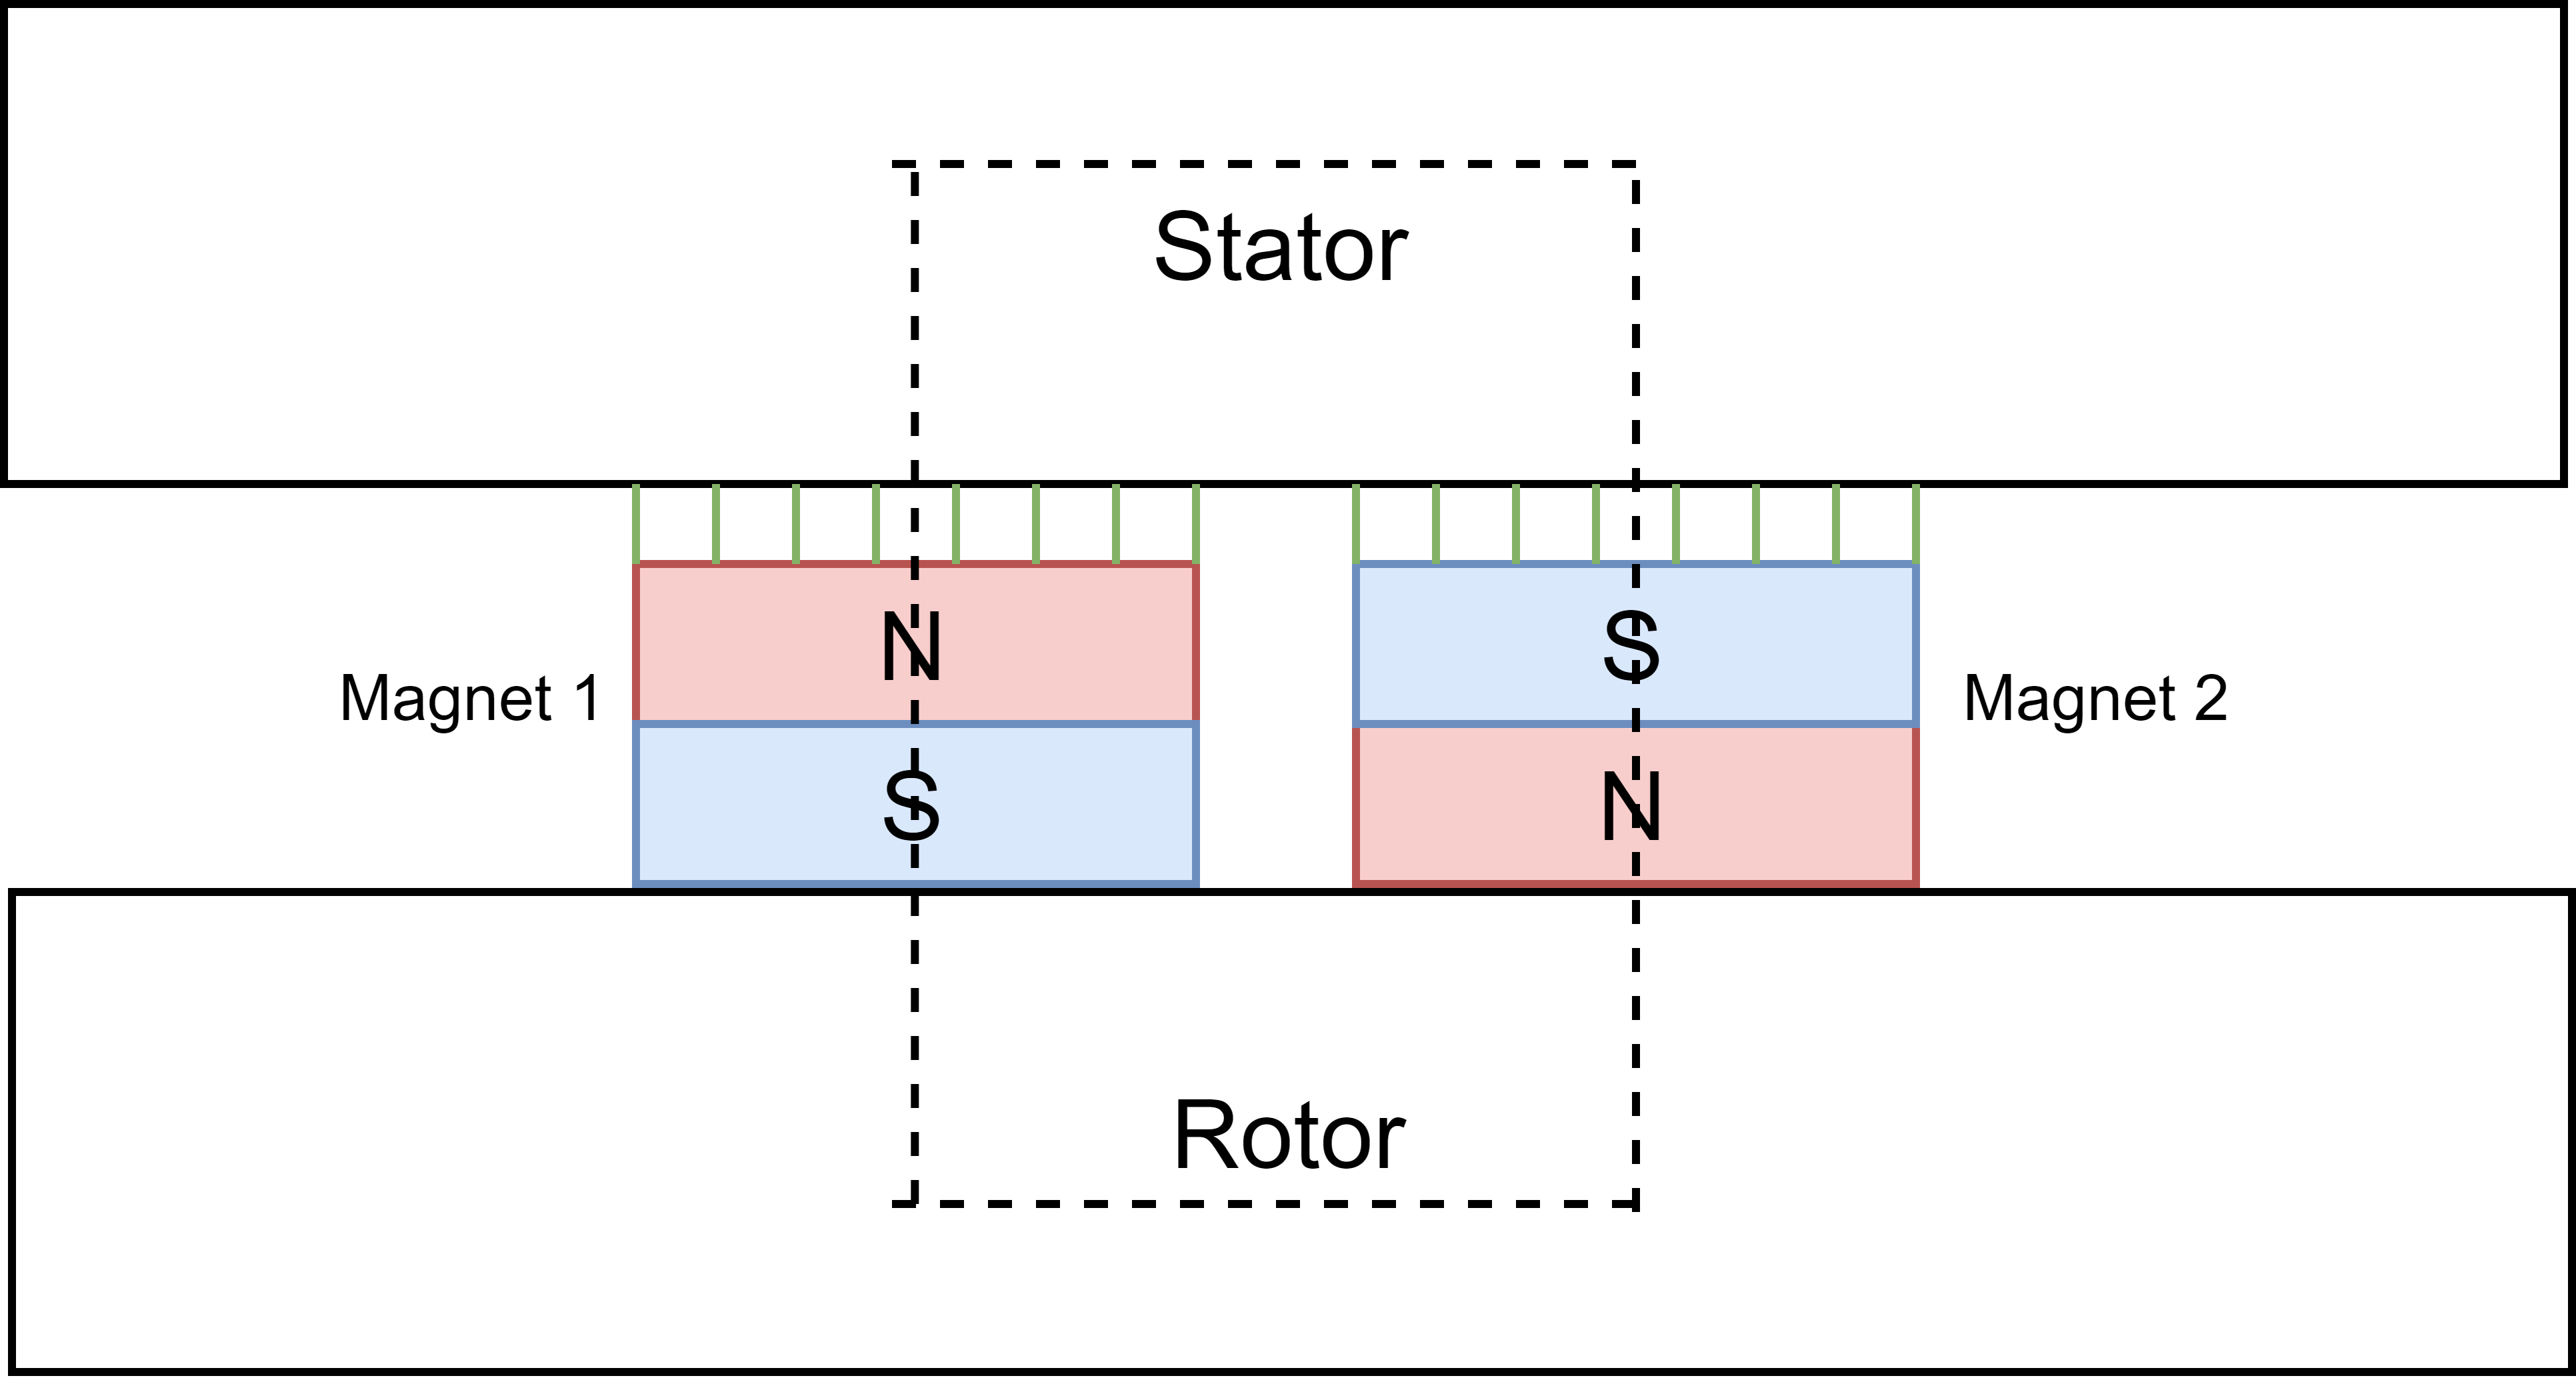
\includegraphics[scale=1.2]{Figures/FluxPath.png}
\caption{Flux Path Through a Pole Pair }
\label{fig:FluxPath}
\end{figure}


\begin{figure}[h!]
\centering
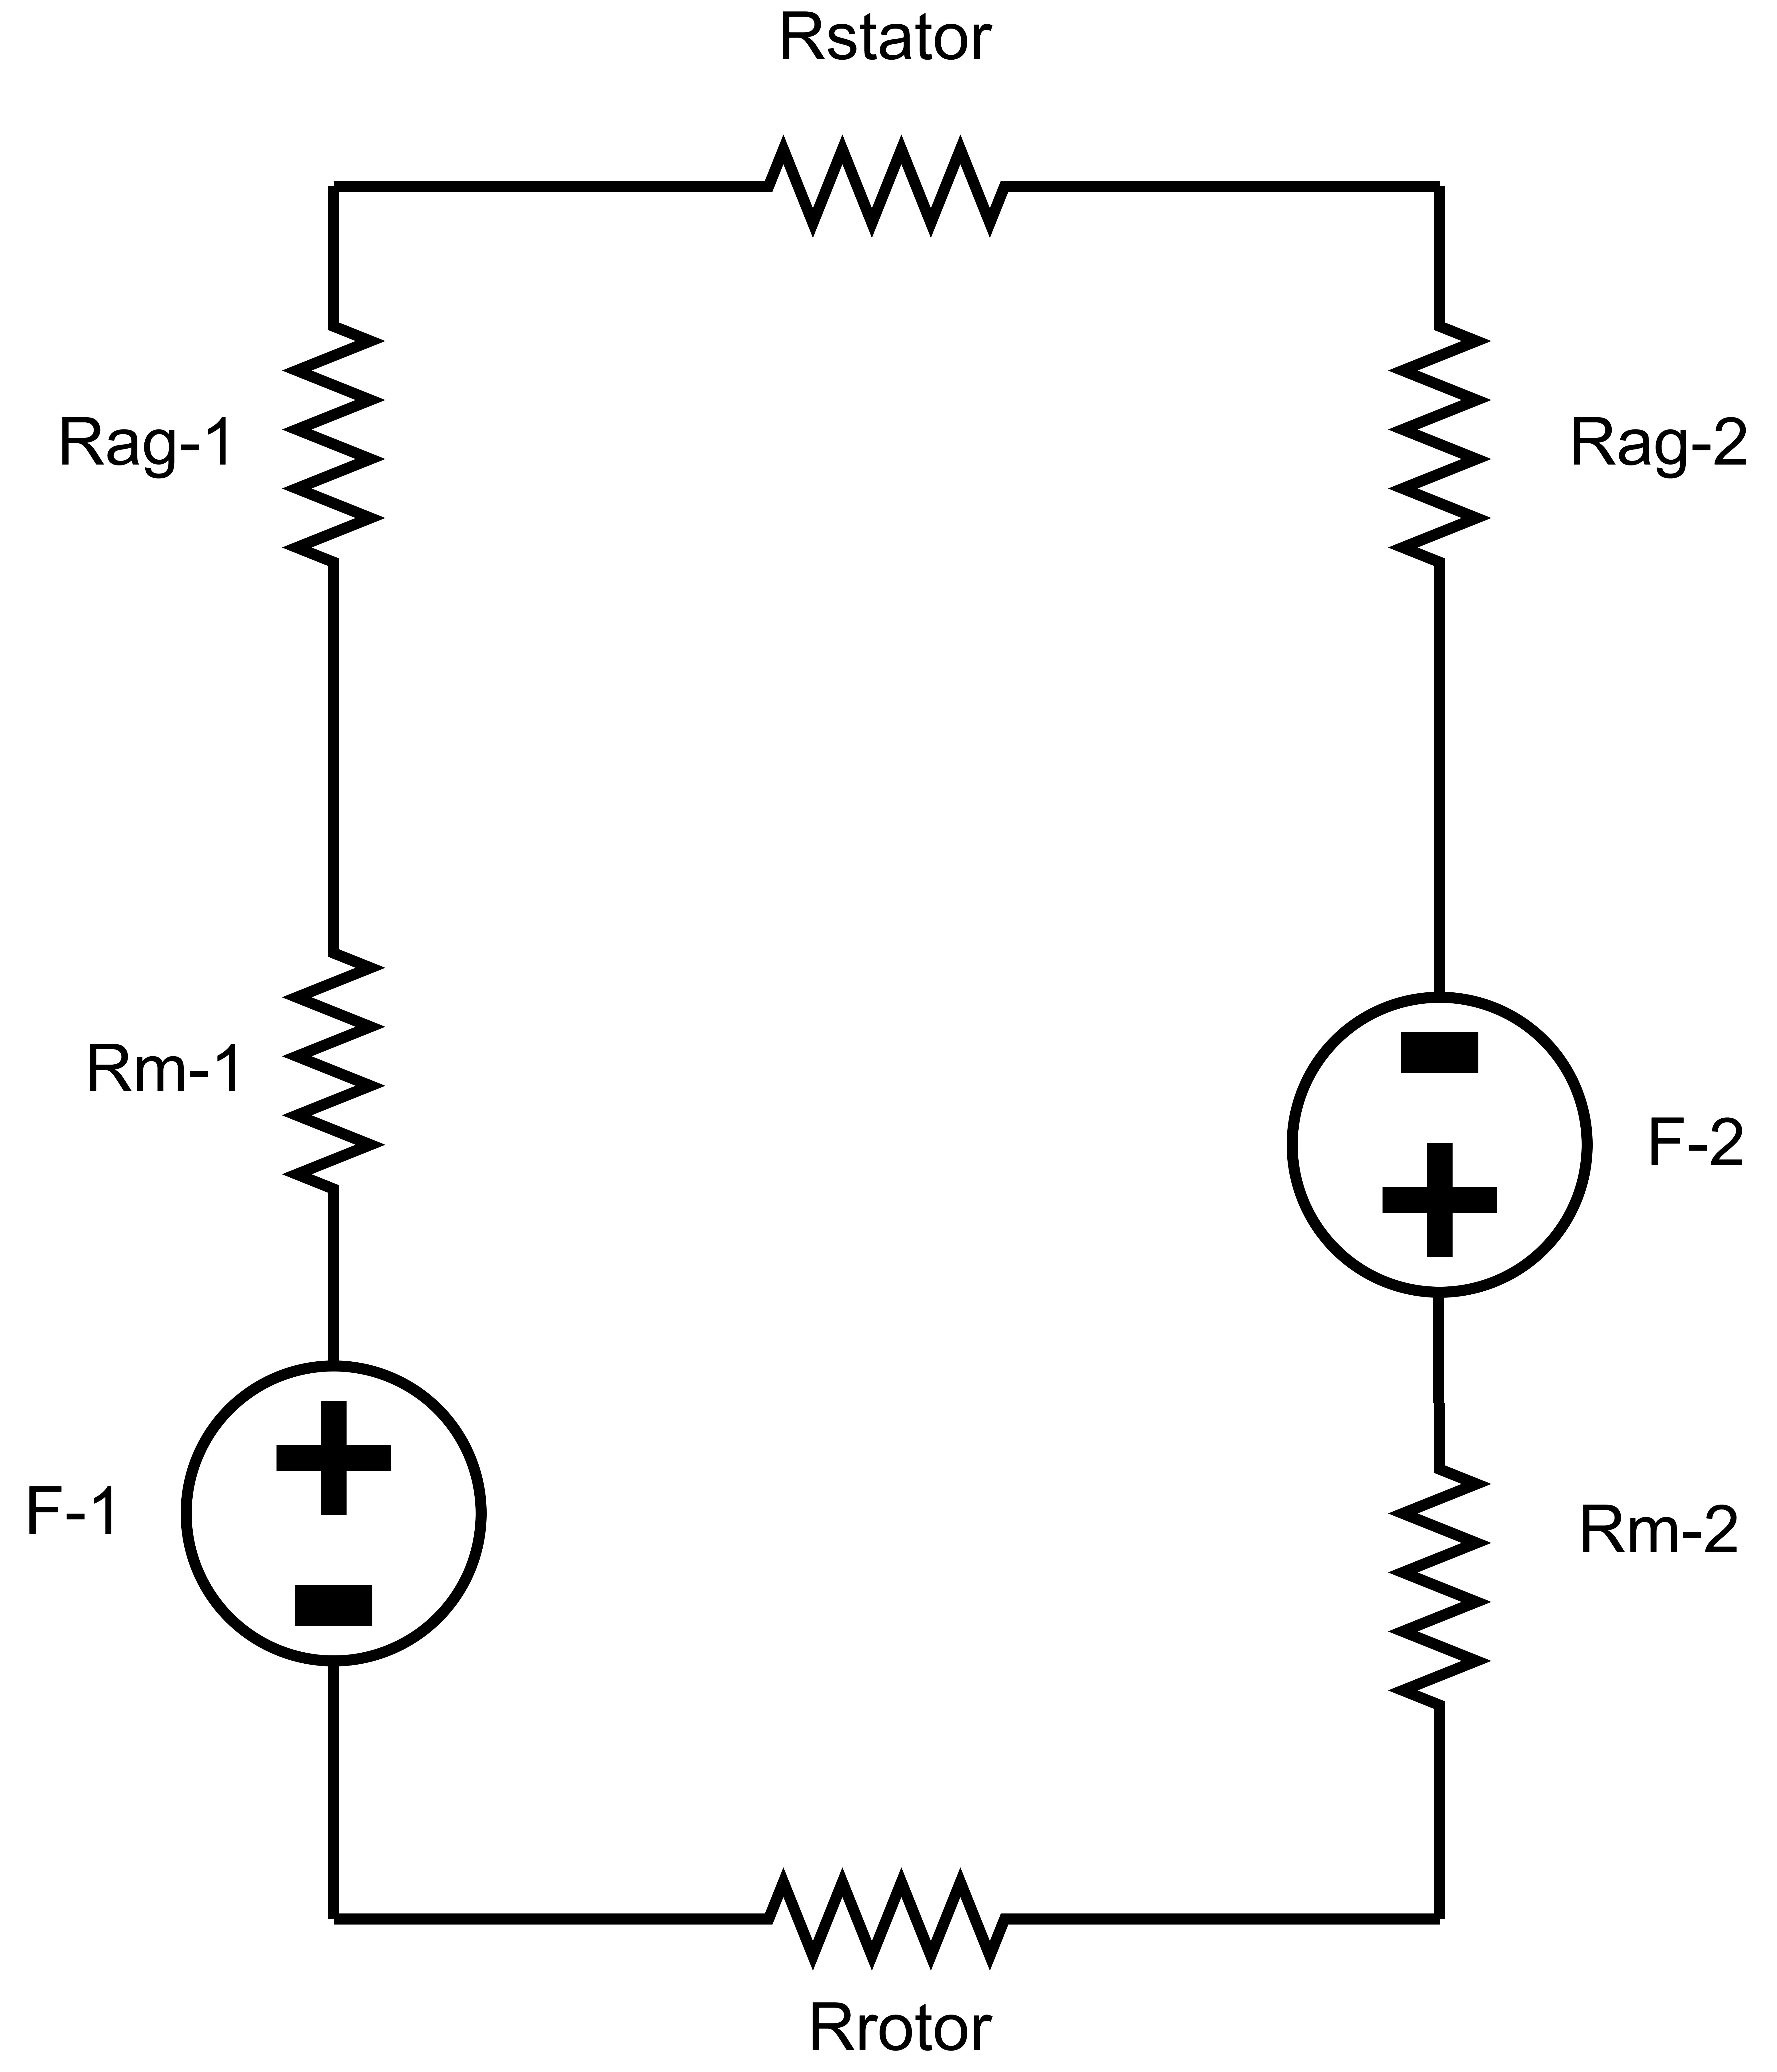
\includegraphics[scale=0.5]{Figures/MagneticCircuit.png}
\caption{Magnetic Equivalent Circuit }
\label{fig:MagneticCircuit}
\end{figure}
\begin{figure}[h!]
\centering
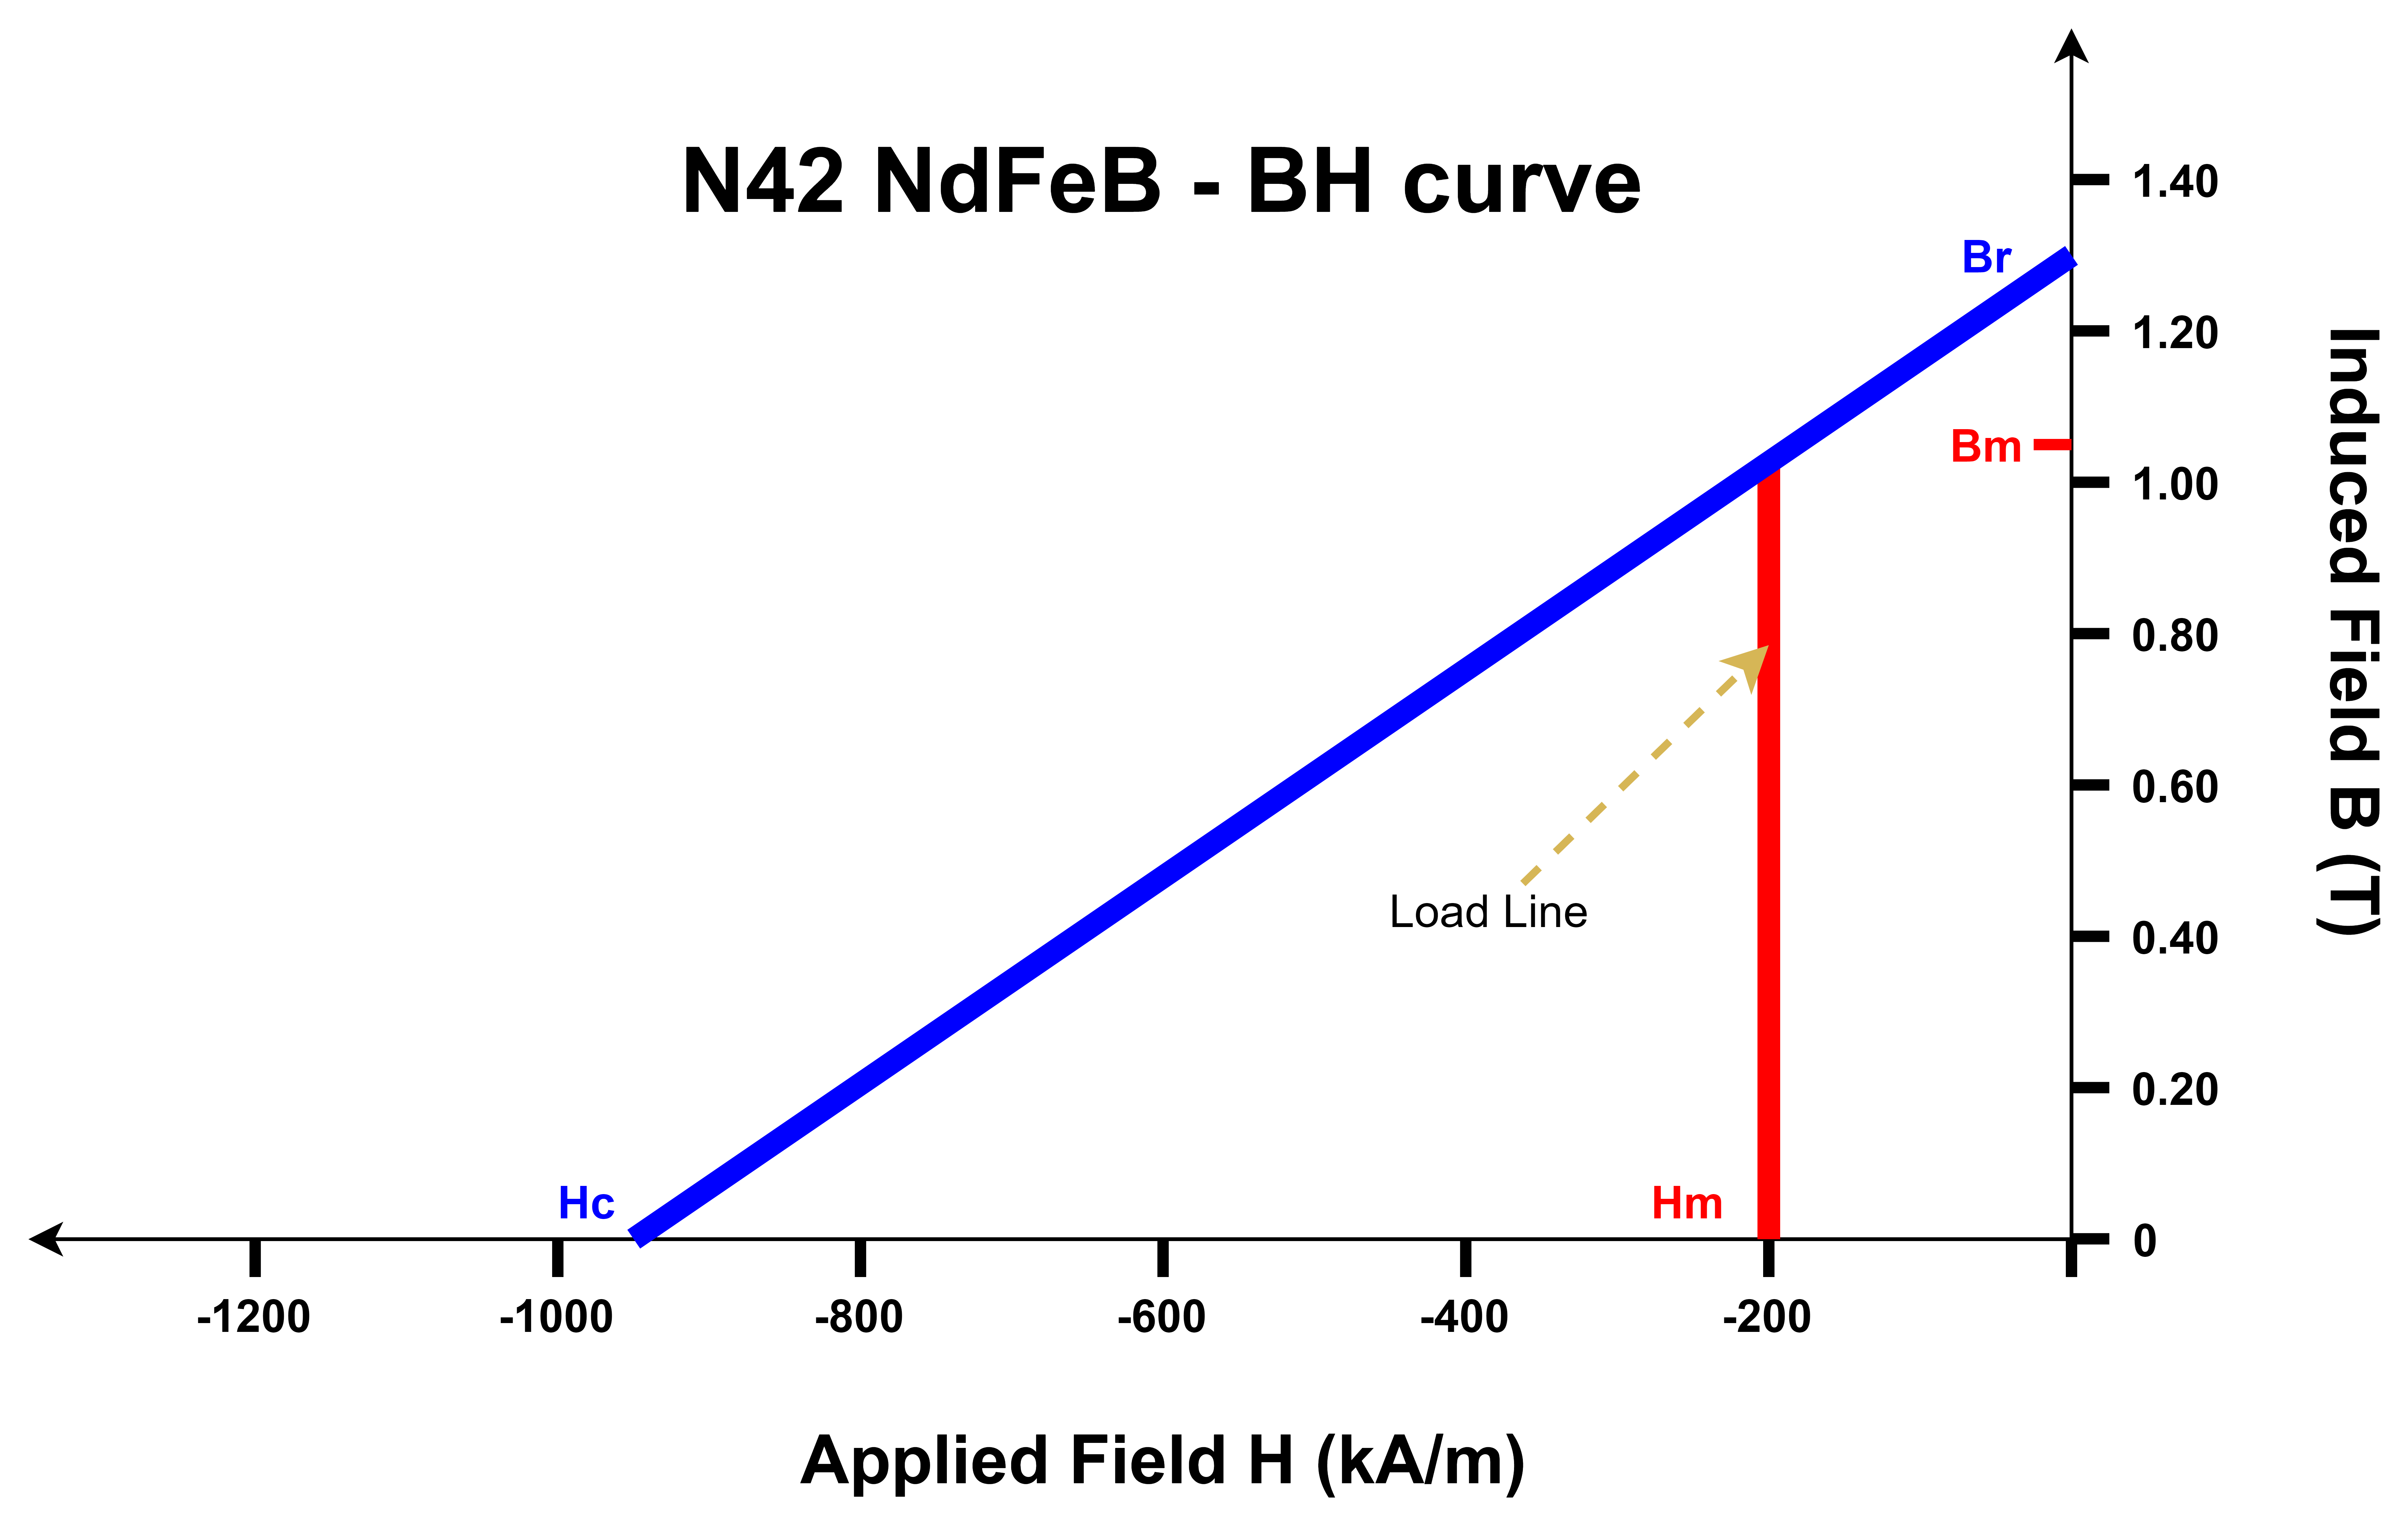
\includegraphics[scale=0.8]{Figures/BHCurve.png}
\caption{N42 NdFeB - BH curve with load line}
\label{fig:BHCurve}
\end{figure}




\bibliographystyle{plain}
\bibliography{references}
\end{document}